%%%%%%%%%%%%%%%%%%%%%%%%%
%% Header for standard beamer presentation
%%
%%  PresentationHeader.tex
%%
%%%%%%%%%%%%%%%%%%%%%%%%%

\documentclass[english,10pt]{beamer}



%%%%%%%%%%%%%%%%%%%%%%%%%%
%% TEMPLATES
%%%%%%%%%%%%%%%%%%%%%%%%%%


% Simple Tabular

%\begin{tabular}{ |c|c|c| } 
% \hline
% cell1 & cell2 & cell3 \\ 
% cell4 & cell5 & cell6 \\ 
% cell7 & cell8 & cell9 \\ 
% \hline
%\end{tabular}





%%%%%%%%%%%%%%%%%%%%%%%%%%
%% Packages
%%%%%%%%%%%%%%%%%%%%%%%%%%



% encoding 
\usepackage[utf8]{inputenc}
\usepackage[T1]{fontenc}


% general packages without options
\usepackage{amsmath,amssymb,amsthm,bbm}

% graphics
\usepackage{graphicx,transparent,eso-pic}

% text formatting
\usepackage[document]{ragged2e}
\usepackage{pagecolor,color}
%\usepackage{ulem}
\usepackage{soul}


% conditions
\usepackage{ifthen}





%%%%%%%%%%%%%%%%%%%%%%%%%%
%% Maths environment
%%%%%%%%%%%%%%%%%%%%%%%%%%

%\newtheorem{theorem}{Theorem}[section]
%\newtheorem{lemma}[theorem]{Lemma}
%\newtheorem{proposition}[theorem]{Proposition}
%\newtheorem{corollary}[theorem]{Corollary}

%\newenvironment{proof}[1][Proof]{\begin{trivlist}
%\item[\hskip \labelsep {\bfseries #1}]}{\end{trivlist}}
%\newenvironment{definition}[1][Definition]{\begin{trivlist}
%\item[\hskip \labelsep {\bfseries #1}]}{\end{trivlist}}
%\newenvironment{example}[1][Example]{\begin{trivlist}
%\item[\hskip \labelsep {\bfseries #1}]}{\end{trivlist}}
%\newenvironment{remark}[1][Remark]{\begin{trivlist}
%\item[\hskip \labelsep {\bfseries #1}]}{\end{trivlist}}

%\newcommand{\qed}{\nobreak \ifvmode \relax \else
%      \ifdim\lastskip<1.5em \hskip-\lastskip
%      \hskip1.5em plus0em minus0.5em \fi \nobreak
%      \vrule height0.75em width0.5em depth0.25em\fi}


%%%%%%%%%%%%%%%%%%%%
%% Idem general commands
%%%%%%%%%%%%%%%%%%%%

%% Commands

\newcommand{\noun}[1]{\textsc{#1}}


%% Math

% Operators
\DeclareMathOperator{\Cov}{Cov}
\DeclareMathOperator{\Var}{Var}
\DeclareMathOperator{\E}{\mathbb{E}}
\DeclareMathOperator{\Proba}{\mathbb{P}}

\newcommand{\Covb}[2]{\ensuremath{\Cov\!\left[#1,#2\right]}}
\newcommand{\Eb}[1]{\ensuremath{\E\!\left[#1\right]}}
\newcommand{\Pb}[1]{\ensuremath{\Proba\!\left[#1\right]}}
\newcommand{\Varb}[1]{\ensuremath{\Var\!\left[#1\right]}}

% norm
\newcommand{\norm}[1]{\left\lVert #1 \right\rVert}



% argmin
\DeclareMathOperator*{\argmin}{\arg\!\min}



%% graphics

% renew graphics command for relative path providment only ?
%\renewcommand{\includegraphics[]{}}




\usetheme{Warsaw}

\setbeamertemplate{footline}[text line]{}
\setbeamercolor{structure}{fg=purple!50!blue, bg=purple!50!blue}

\setbeamercovered{transparent}

\setbeamertemplate{footline}[frame number]
\setbeamertemplate{navigation symbols}{}


% shortened command for a justified frame
%\newcommand{\jframe}[2]{\frame{\frametitle{#1}\justify{#2}}}


%\newcommand{\jitem}[1]{\item \begin{justify} #1 \end{justify} \vfill{}}
\newcommand{\sframe}[2]{\frame{\frametitle{#1} #2}}



\newcommand{\indep}{\rotatebox[origin=c]{90}{$\models$}}



\usepackage{tikz}

\usepackage{multirow}


\usepackage{mdframed}

% in the case of ps graphics : convert ps to pdf
%\usepackage[usenames,dvipsnames]{pstricks}
%\usepackage{auto-pst-pdf}


%\usepackage[dvipsnames]{xcolor}
\usepackage{xcolor}


\makeatother



%%%%%%%%%%%%%%%%%%%%%
%% Begin doc
%%%%%%%%%%%%%%%%%%%%%

\begin{document}


\title{Methods for the exploration of simulation models}


\author{OpenMOLE Team$^{1}$}

\institute{$^{1}$UPS CNRS 3611 ISC-PIF}


\date{Dynamicity meeting\\
Lyon, 21/06/2018
}


%%%%%%%%%%%%%%%%%%%%%%%%%%%%%%%%
\begin{frame}
\titlepage
\end{frame}

%\begin{frame}
%\tableofcontents
%\end{frame}
%%%%%%%%%%%%%%%%%%%%%%%%%%%%%%%%


\sframe{Research projects}{

\textbf{Sensitivity analysis:}
\begin{itemize}
	\item Robustness of calibration algorithms to stochasticity
	\item Sensitivity of models to the spatial configuration
\end{itemize}

\bigskip

\textbf{LUTI models:}

\begin{itemize}
	\item Testing Luti models against stylized facts
	\item Luti toy-model : the Lutecia model
	\item Analysis of scenarios
\end{itemize}

}

\sframe{Robustness to stochasticity}{

	\textit{How must a stochastic fitness be handled in GAs ? (number of repetitions, statistical robustness of the estimation, form of the Pareto front)}
	
	\bigskip
	
	$\rightarrow$ OpenMOLE has developed its own original method based on dimension embedding
	
	\bigskip
	
	\textbf{Objectives :}
	
	\begin{itemize}
		\item More thorough benchmark of the evaluation strategy
		\item Study of unconventional noise landscapes, found in ``real'' models
		\item Test on different case studies
\end{itemize}		
	
}



\sframe{Sensitivity of spatial models}{
	
% Analyse de sensibilité à la configuration spatiale

%    Générateur de réseaux de transport
%    Générateur de grilles spatiales (population/emplois)
	
	\textit{Sensitivity of models with a spatial component mostly ignore the effect of the spatial configuration}

	\medskip
	
	$\rightarrow$ How to control with synthetic configurations ?
	
	\medskip
	
	$\rightarrow$ How to test the sensitivity to missing data or spatial uncertainty ?
	
\bigskip
\bigskip	
	
	\textbf{Objectives:}
	\begin{itemize}
		\item Synthetic spatial configuration generators embedded into OpenMOLE (grid and networks)
		\item Perturbations of real geographical data
		\item Associated methods and measures
\end{itemize}		
	
	
}

\sframe{Sensitivity of spatial models}{
	
	\textit{Generation of spatial population grids \cite{cottineau2017initial} \cite{raimbault2017calibration}}
	
	\medskip
	
	\centering	
	
	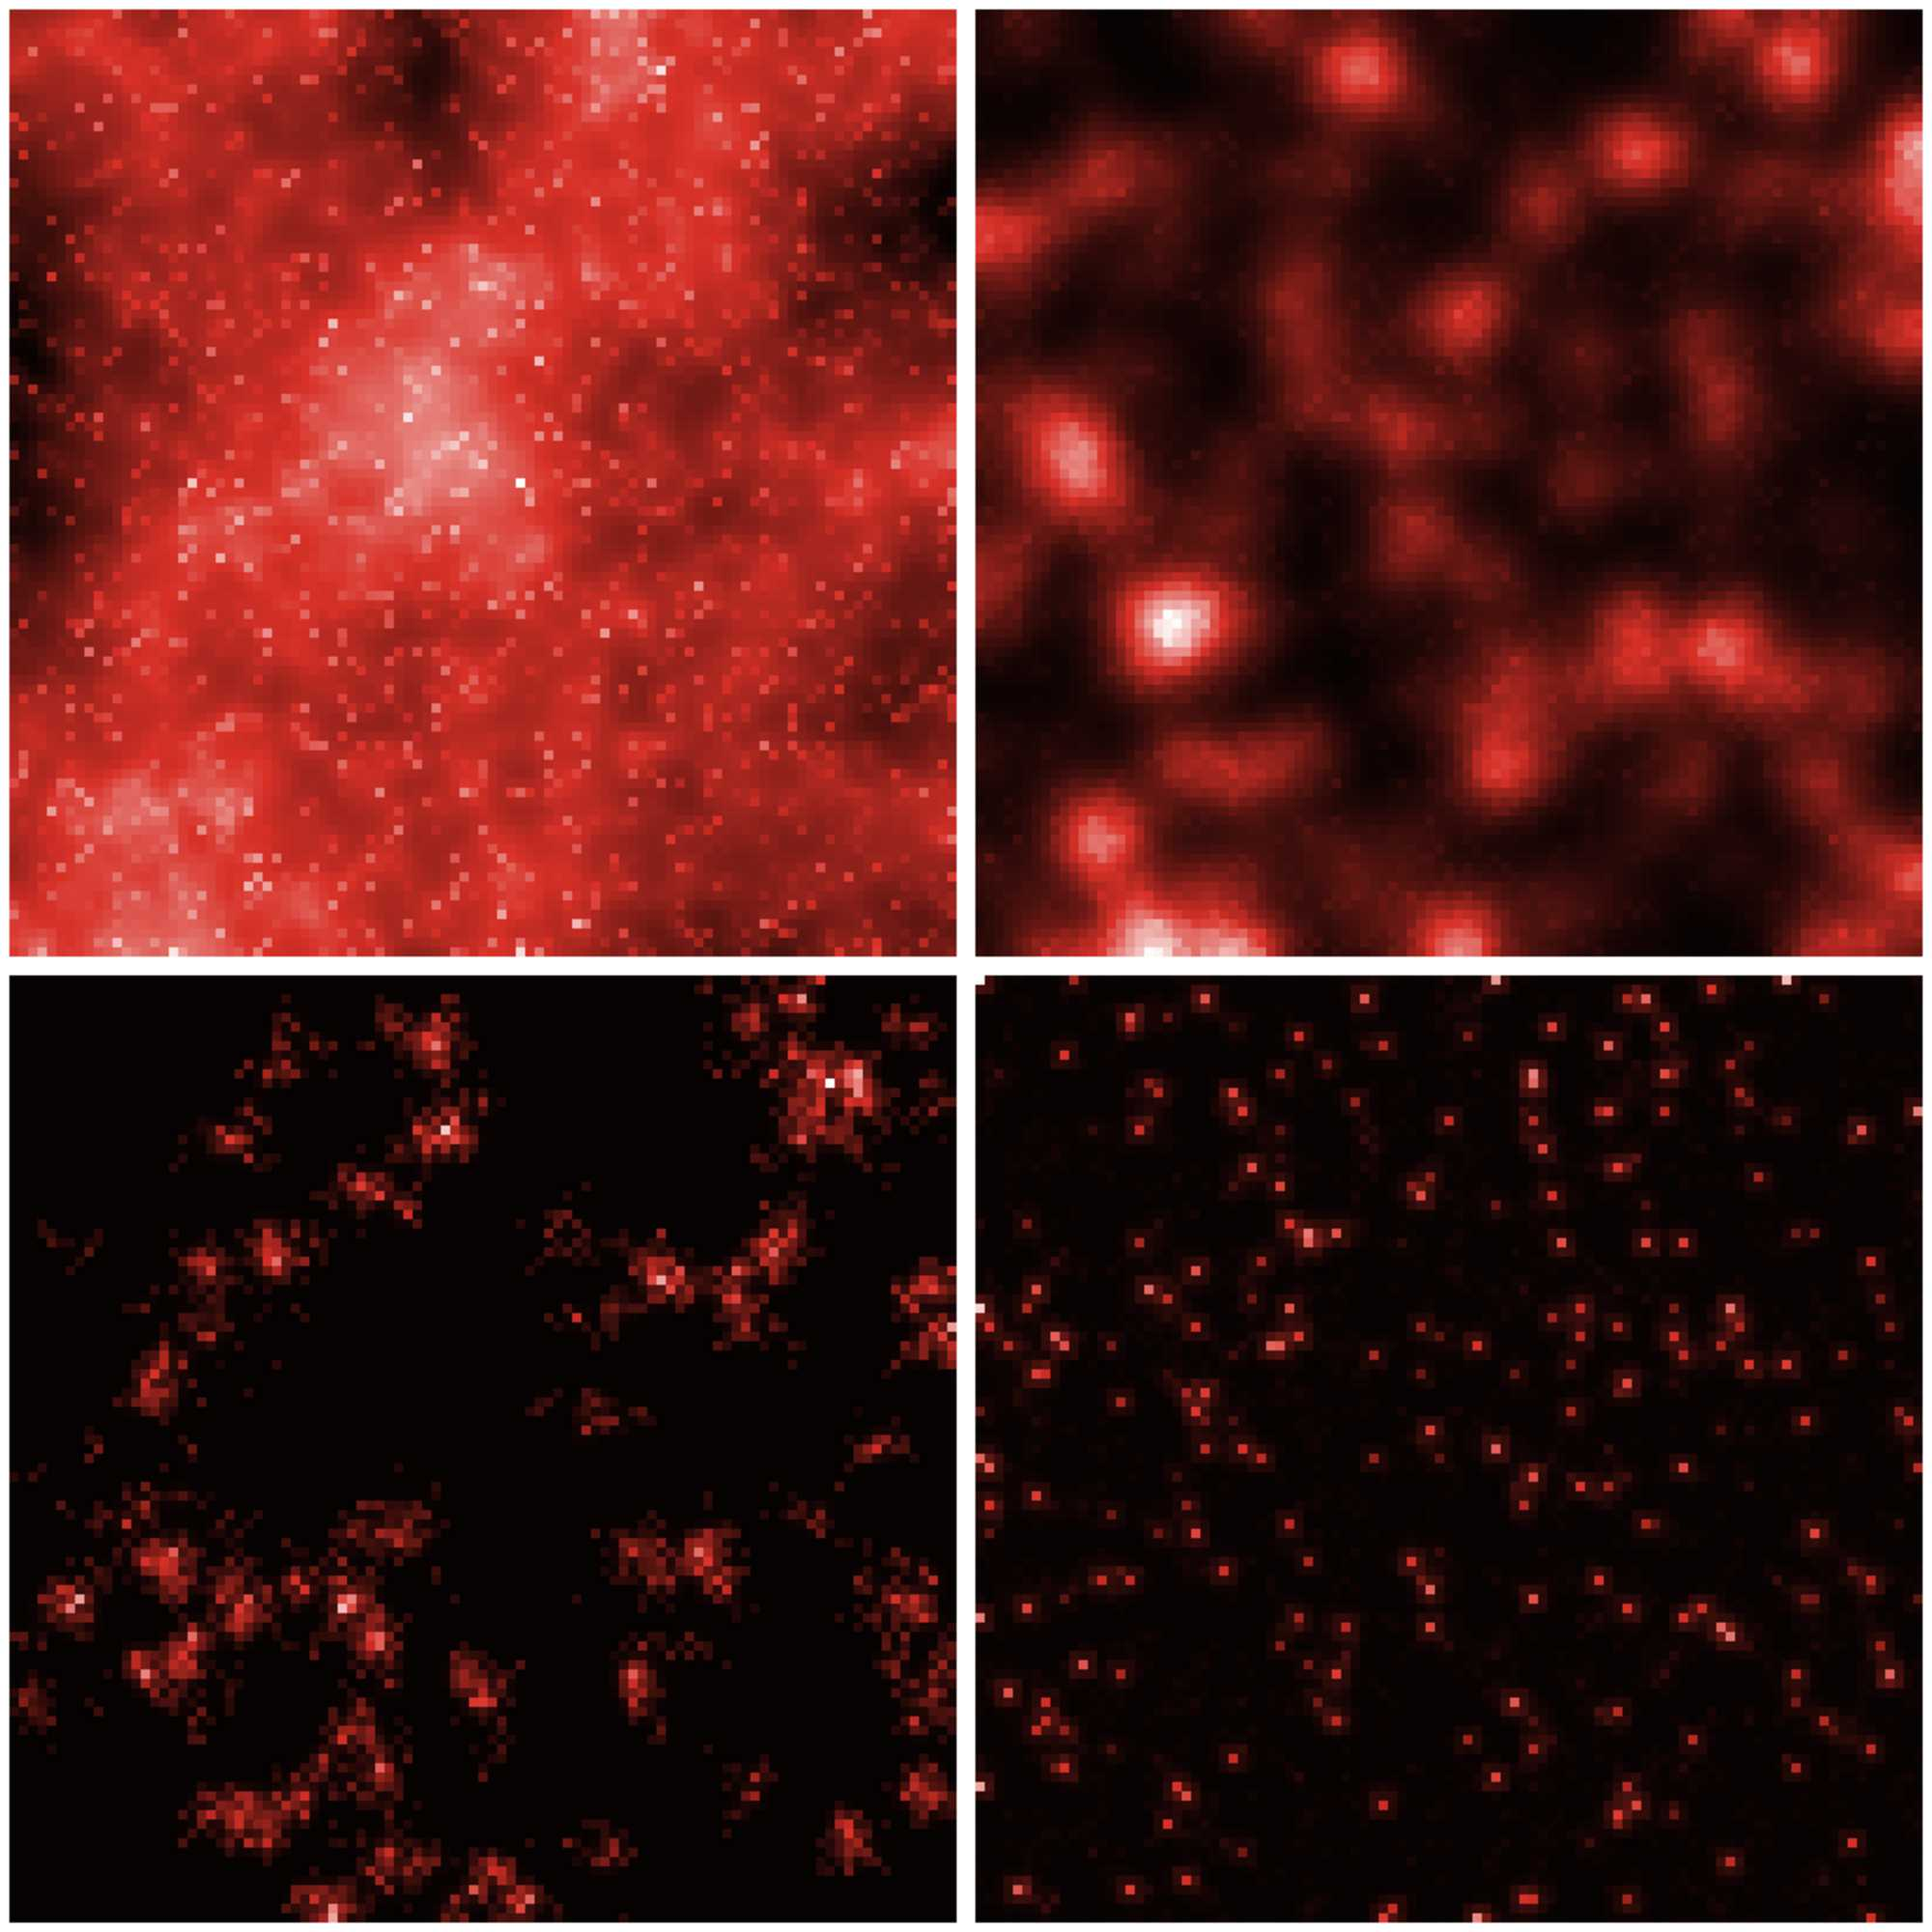
\includegraphics[height=0.8\textheight]{figures/5-2-2-fig-density-fig2.jpg} 
	
		
	
}

\sframe{Sensitivity of spatial models}{
	
	\textit{Generation of road network by multimodeling \cite{raimbault2018multi}}
	
	\medskip
	
	\centering	
	
	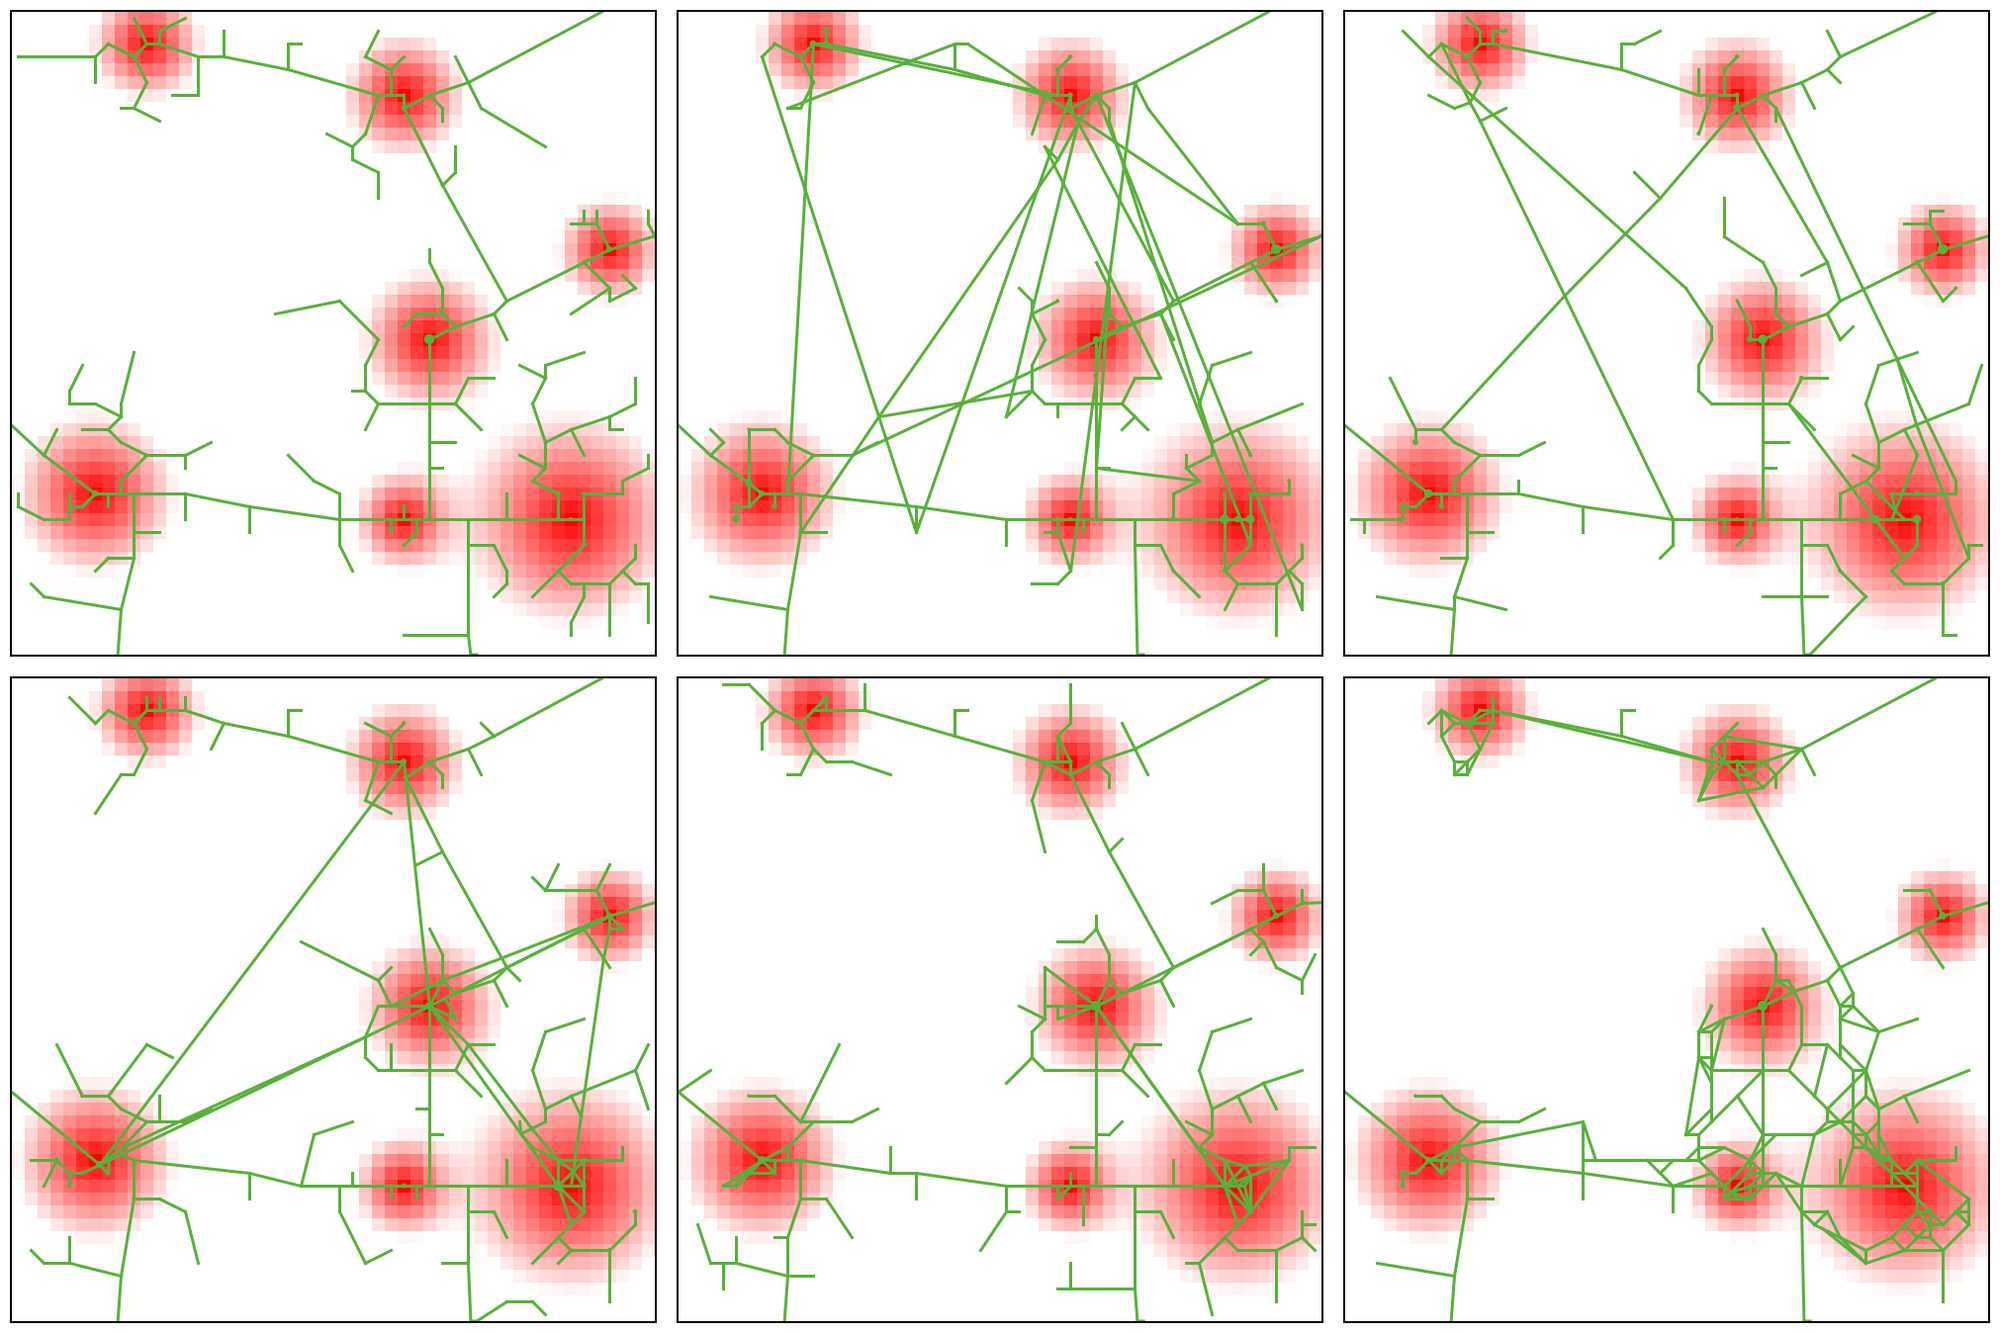
\includegraphics[height=0.8\textheight]{figures/7-1-2-fig-networkgrowth-examples.jpg} 
	
			
	
}





\sframe{Stylized facts in Luti models}{
	
	\textit{How to validate a Luti model ?}

	\bigskip
	
	$\rightarrow$ Development of a generic method to test the validity of a model against stylized facts (Guillaume)
	
	\bigskip
	
	$\rightarrow$ List of stylized facts for Luti models from the literature (cf A. Bonnafous: \textit{Is the model better than nothing ?} : very difficult constraint !)
	
		
	
}



\sframe{Luti toy model}{

	\textit{The Lutecia model \cite{le2015modeling}: coupling a Luti with endogenous transportation growth to model the co-evolution of networks and territories}

	$\rightarrow$ Redevelopment in scala as a toy model for the test of methods
	
	\medskip
	
	\centering	
	
	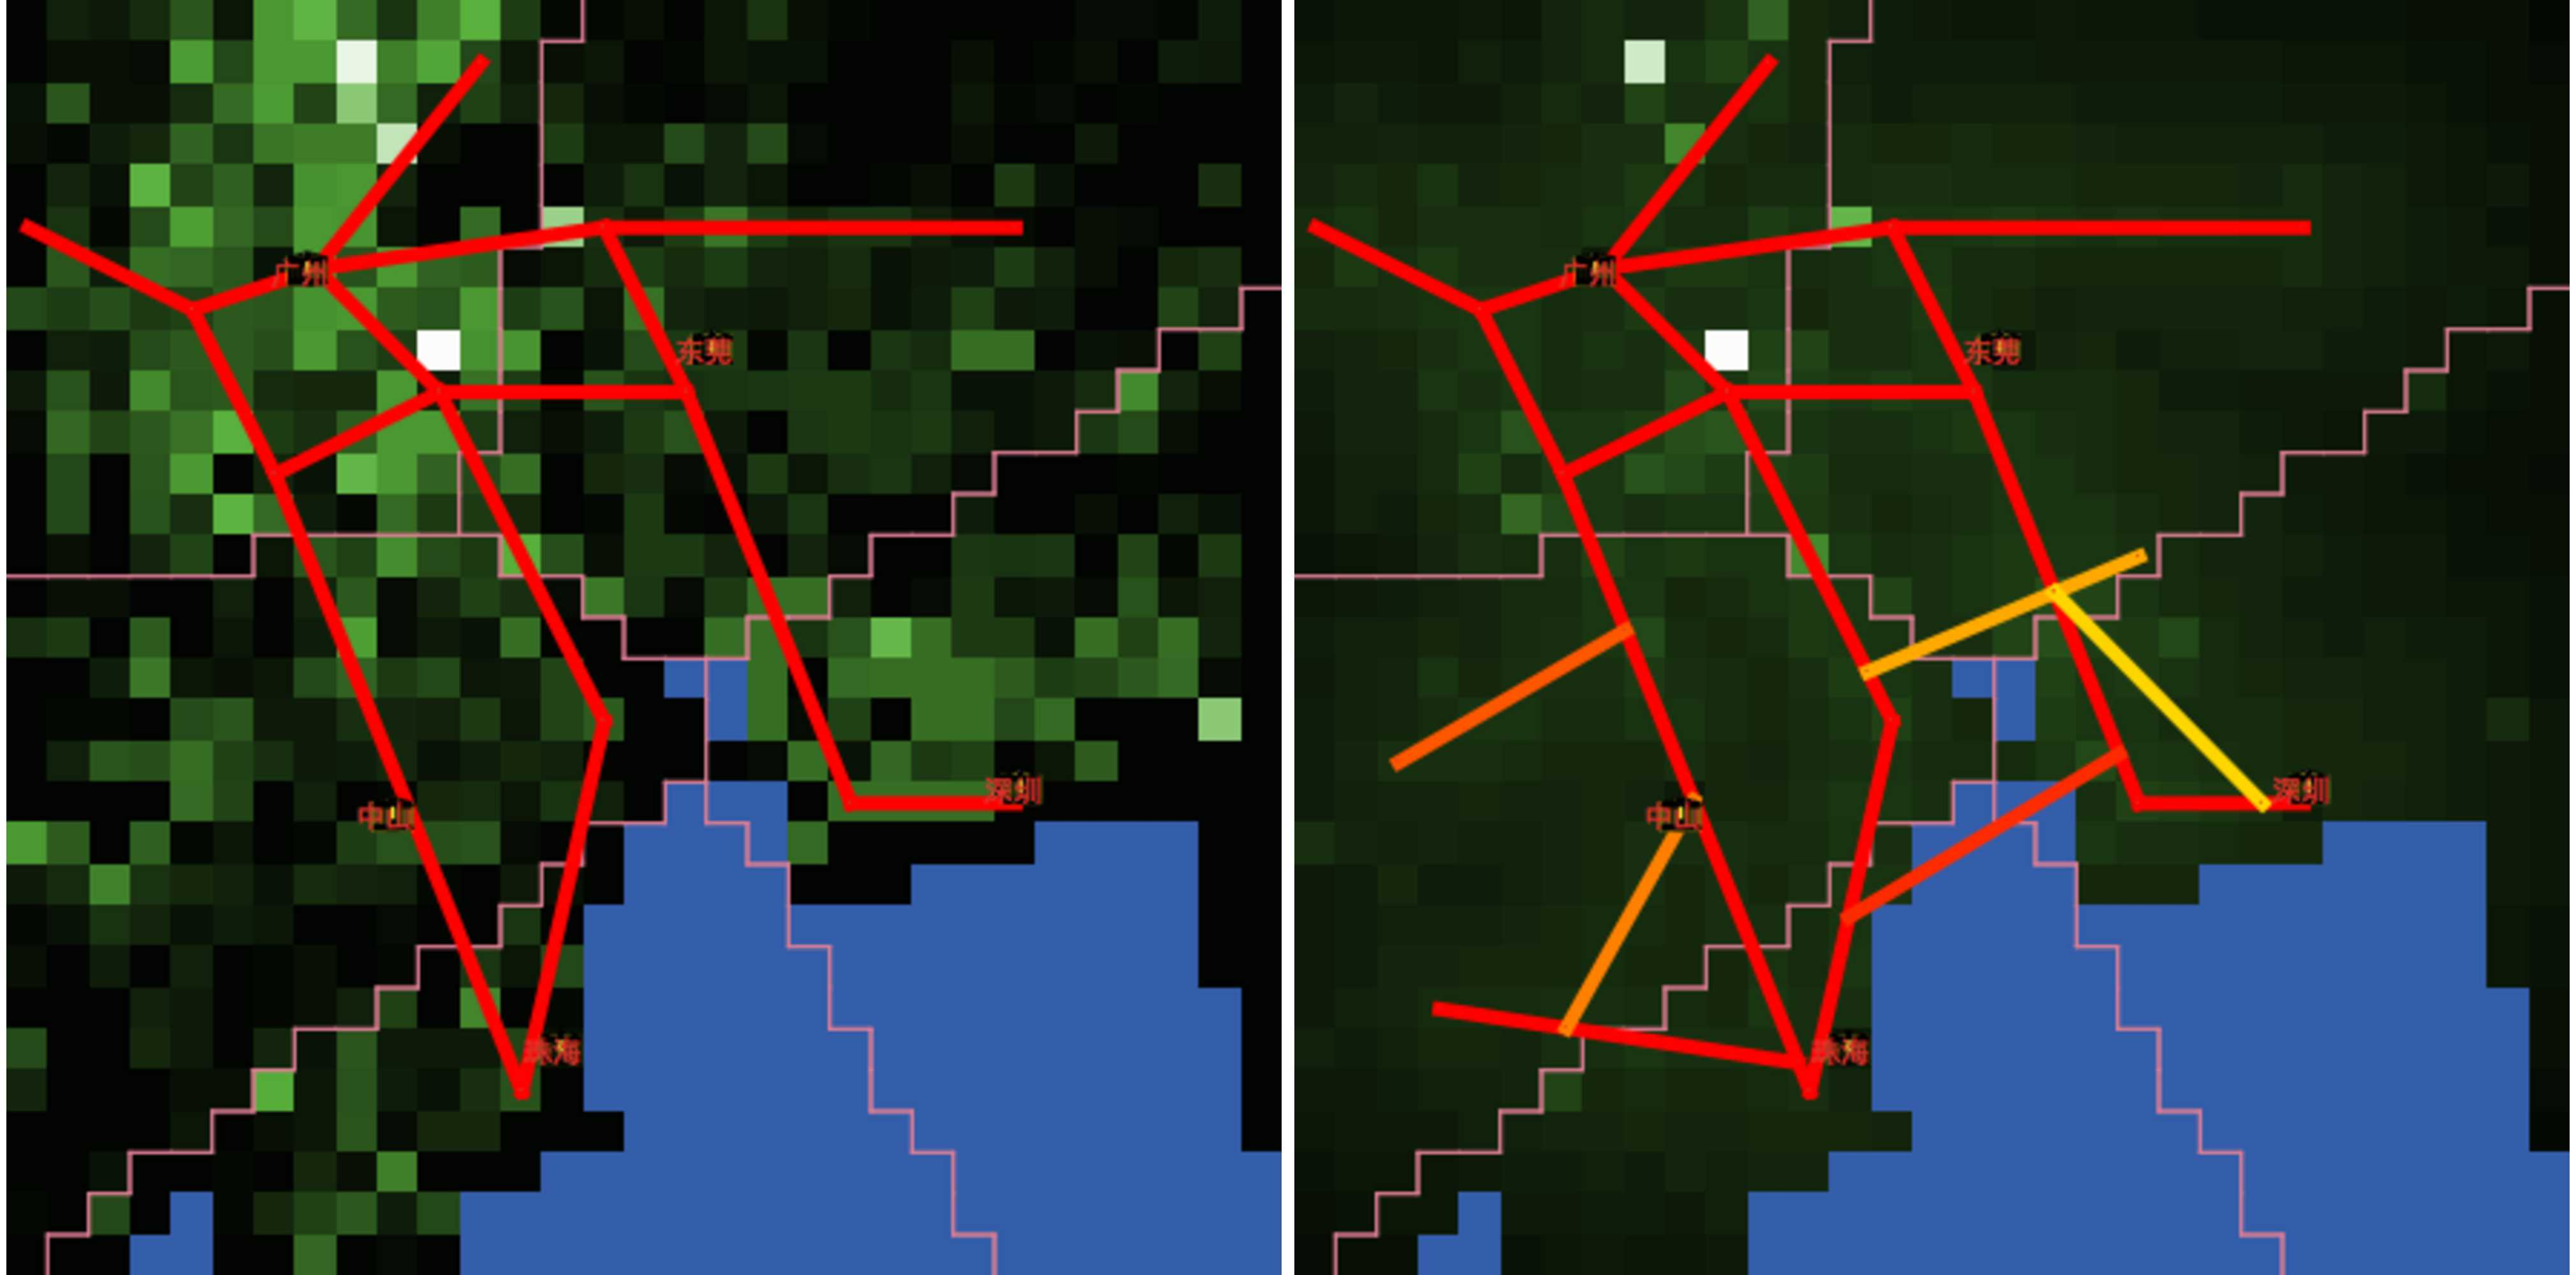
\includegraphics[height=0.65\textheight]{figures/7-3-3-fig-lutecia-ex-prd.jpg}
		
	
}



\sframe{Analysis of scenarios}{

\textit{Comparison of scenarios for transportation networks}

\medskip

\centering

	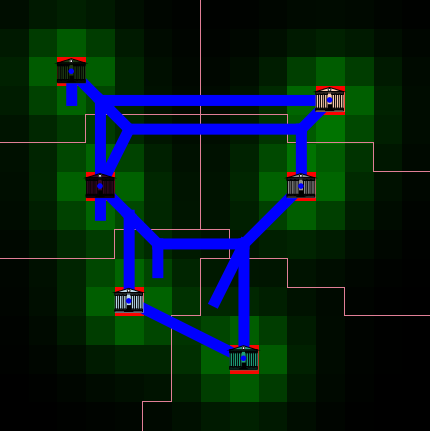
\includegraphics[width=0.3\textwidth]{figures/bionw_territ6_gamma1_1_bis.png}
    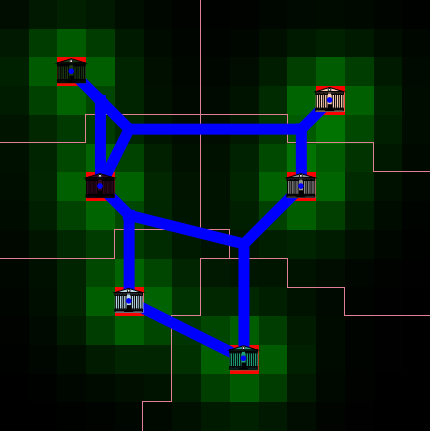
\includegraphics[width=0.3\textwidth]{figures/bionw_territ6_gamma1_2_quart.png}
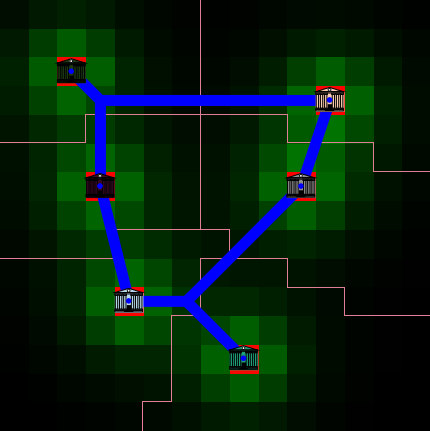
\includegraphics[width=0.3\textwidth]{figures/bionw_territ6_gamma1_3_bis.png}\\\smallskip
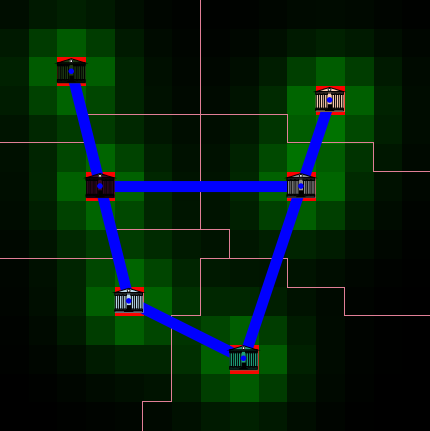
\includegraphics[width=0.3\textwidth]{figures/bionw_territ6_gamma1_5.png}
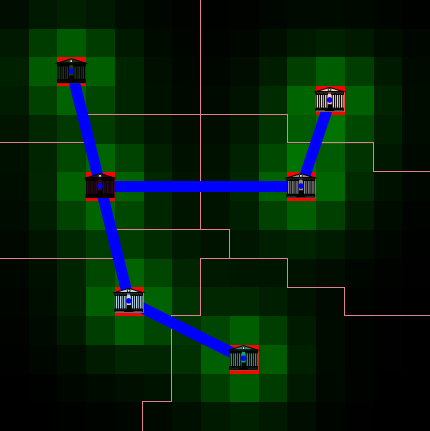
\includegraphics[width=0.3\textwidth]{figures/bionw_territ6_gamma1_8.png}
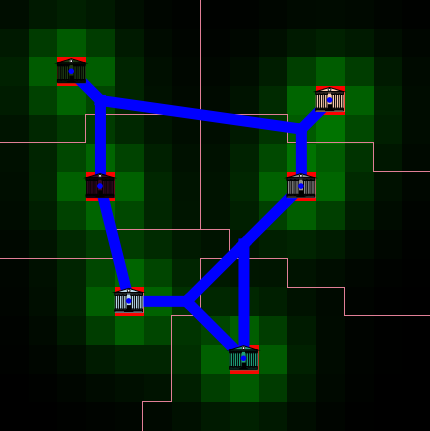
\includegraphics[width=0.3\textwidth]{figures/bionw_territ6_gamma1_25_bis.png}
}

\sframe{Analysis of scenarios}{
	
	\textit{Performance of generated synthetic networks}
	
	\medskip	
	
\centering	
	
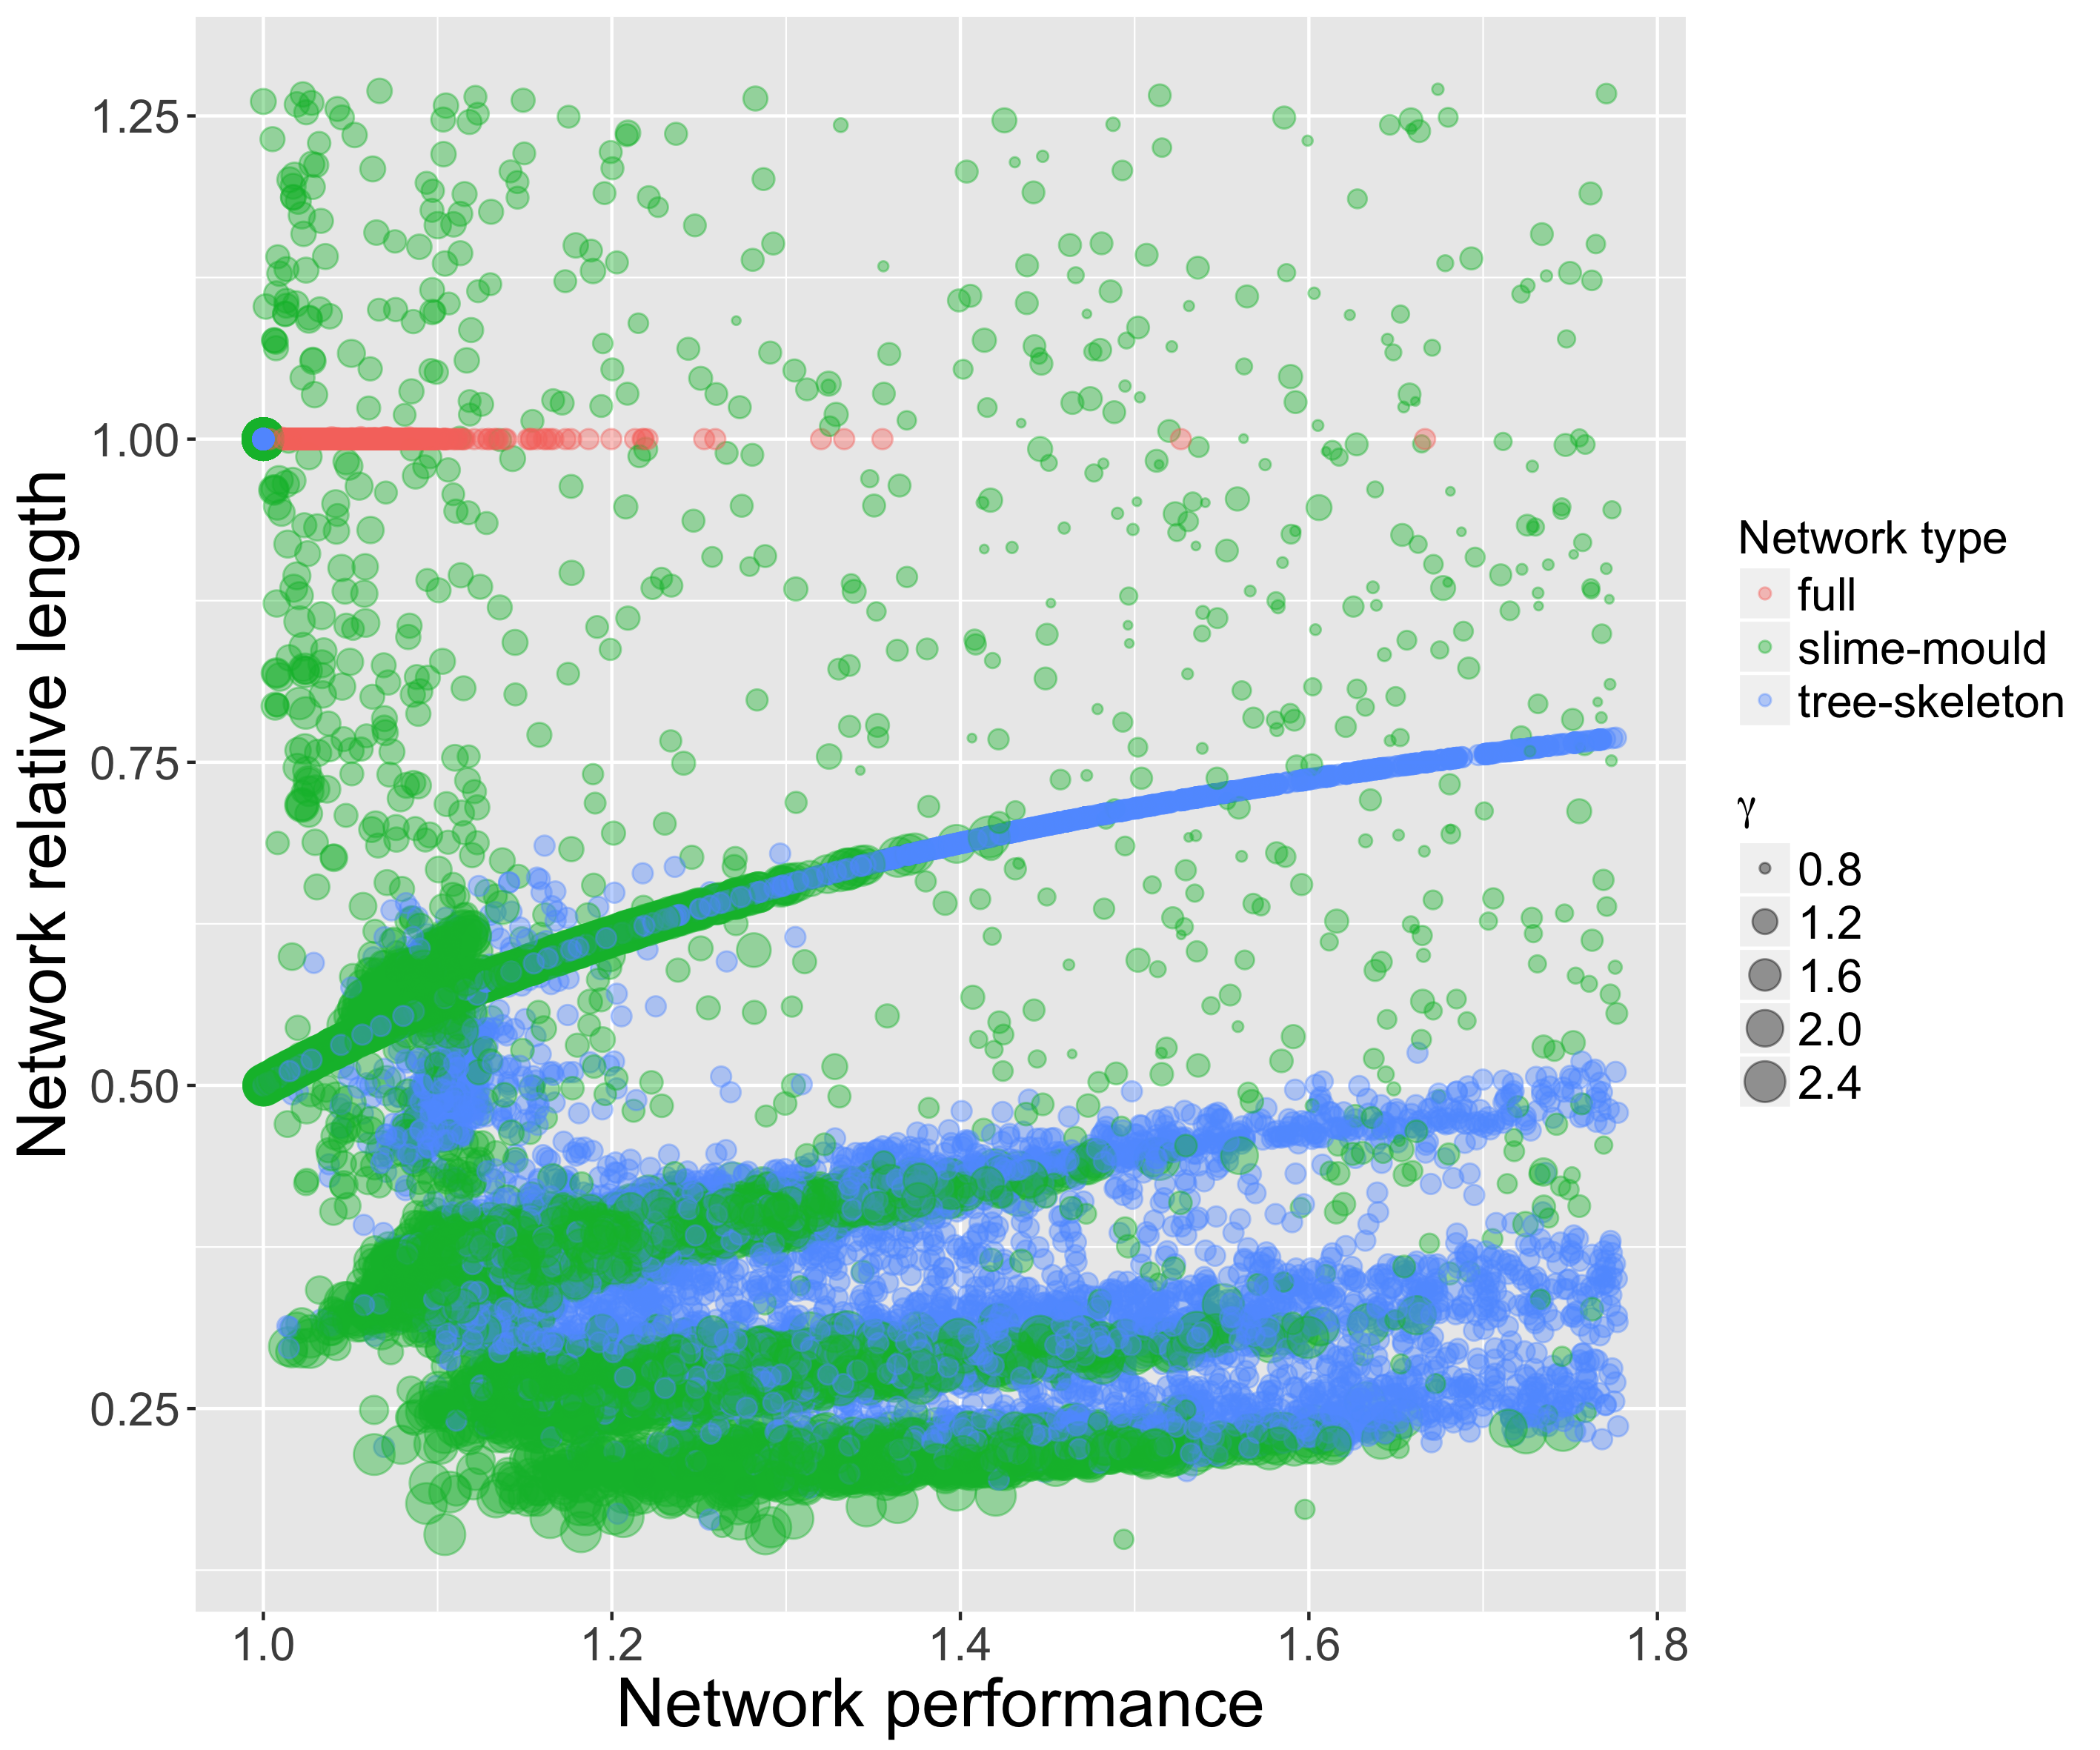
\includegraphics[height=0.8\textheight]{figures/paretoSpeedLength.png}
	
}





%%%%%%%%%%%%%%%%%%%%%%%%%%%%%%%%
\begin{frame}[allowframebreaks]
\frametitle{References}
\bibliographystyle{apalike}
\bibliography{biblio.bib}
\end{frame}
%%%%%%%%%%%%%%%%%%%%%%%%%%%%%%%%


\end{document}